\documentclass{article}
\usepackage[utf8]{inputenc}
\usepackage{amsmath}
\usepackage{listings}

\usepackage{amsthm}
\usepackage{graphicx}
\usepackage{upgreek}
\usepackage{algorithm}
\usepackage{algpseudocode}


\date{04 February 2019}
\marginparwidth 0.5in 
\oddsidemargin 0.25in 
\evensidemargin 0.25in 
\marginparsep 0.25in
\topmargin 0.25in 
\textwidth 6in \textheight 8 in
\newtheorem{question}{Question: }
\theoremstyle{case}
\newtheorem{case}{Case}
\graphicspath{ {images/} }
\begin{document}
\author{Sai Vineet Reddy Thatiparthi}

 \title{%
  Advanced Machine Learning \\
  \large Homework 1}
\maketitle
\textbf{The program is attached along with the submission. One has to enter the degrees of the polynomial after the program is run in the following format - 1 5 10 50. It is written in Python3.}
\begin{enumerate}
    \item [A.] \textbf{Use a polynomial estimator of degree 1, 5, 10, and 50. Plot the
function that you obtain with each of the polynomials overlaid on
the data}
\end{enumerate} 
\begin{proof} 
I have attached the code the runs the polynomial estimator as well as plots the resultant function on the data. The user has to enter the degrees of the polynomial that needs to be estimated.
\end{proof}

\begin{enumerate}
    \item [B.] \textbf{Plot the MSE obtained on the training data and the test data as
a function of the degree of the polynomial}
\end{enumerate}
\begin{proof}
The MSE of the different polynomials will be displayed at the bottom of the plotted functions on the graph itself. These graphs are also the same graphs as sub-question D.

\end{proof}
\begin{enumerate}
    \item [C.] \textbf{Based on the above experiments, what can you say about the
degree of the polynomial and the MSE}
\end{enumerate} 
\begin{proof} 
It seems that with the increase in the degree of the polynomial, the MSE reduces when one is calculating the MSE on the training set. When it comes to prediction (testing set), the MSE of polynomials with low and high degrees was quite high. However, when one chooses a polynomial whose degree is not very high nor very low ('just right') have the least MSE on the testing set. This is because such models with just the right degree polynomial, the bias and the variance are low enough that the MSE is optimal. \\ \\
This is also the basic concept of underfitting and overfitting.
\end{proof}

\begin{enumerate}
    \item [D.] \textbf{Plot the MSE, the squared Bias, and the Variance as a function
of the degree of the polynomial. Comment on what you observe}
\end{enumerate} 
\begin{proof}
The output graphs of this question are the same as that of sub-question B.\\ \\
The MSE first reduces and then keeps increasing. When the degree of the polynomial is low, it seems like the estimator has a high bias but this bias reduces with increase in the degree.\\ \\ The variance, on the other hand, was very low when the estimator's degree was low. However, with increase in the degree, the variance, too, increased. So, with increase in Bias, the variance reduced and with increase in variance, the bias reduced. The MSE is the sum of of the bias squared and the variance, so in the end, it looked like this - 
\end{proof}
\begin{enumerate}
    \item [E.] \textbf{Create a new estimator whose output is the average of the 4 estimators you created above (i.e. polynomials of degree 1, 5, 10,
and 50). Plot the function that you obtain overlaid on the data.
What is the difference between this (composite) estimator and the
individual estimators that you created?}
\end{enumerate} 
\begin{proof} 
The graphs are available at the end of the program run. They are titled as Composite polynomial. \\ \\
The composite estimator did not perform as well as an estimator whose degree was somewhere near 5. This could possibly be because it was influenced by the 50 degree polynomial, which has a very high MSE on the training set as it was overfit. However, it did not perform as bad as the 50 degree polynomial or the 1 degree polynomial as its performance was normalised by the other order polynomials. The graph looked something like this - 
\begin{figure}[h]
            \caption{Average polynomial's performance}
            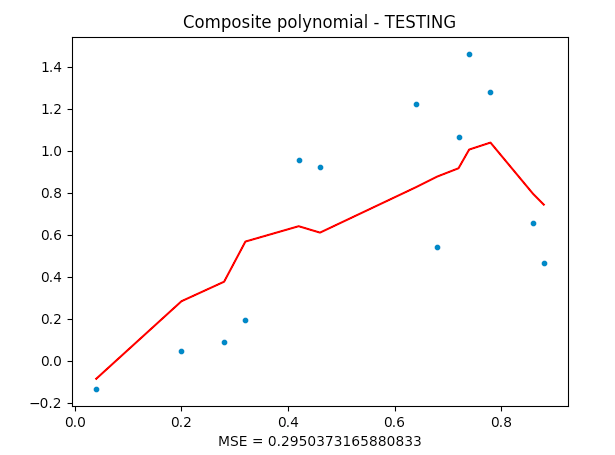
\includegraphics[scale=0.4,width=\textwidth]{n3.png}
            % \centering
            \end{figure}
\end{proof}
\begin{enumerate}
    \item [F.] \textbf{A colleague suggested the following – create a 100 estimators and
take the 3 best estimators from them (possibly in terms of MSE
on the training data). Use the average of the 3 best estimators to
create a new estimator. Comment on the performance you would
expect to see from this estimator. Be very specific.}
\end{enumerate} 
\begin{proof} 
Let's say that there is a class of 100 students. During school hours, a teacher asked the students one question. The teacher then noted down the answers of the three best students in the class - and then observed that all of them were the same. The same analogy can be applied to our problem - replacing the students with estimators. Despite one using the three best estimators and then creating a new estimator out of their average, the output of this estimator will not be any different from the three best estimators. Their accuracy and error will be almost the same, and not any better. This is only because we are just averaging the best estimators and they are best only because the accuracy could not be increased anymore - even averaging them out will not change this.
\end{proof}

\end{document}